\documentclass[landscape]{jhuslides3C}
\usepackage{url}
\usepackage{amsmath}
\usepackage{graphicx}
\usepackage{color}
\usepackage{colortbl}
\usepackage{epic,ecltree}
%\usepackage{bar}
% \usepackage{eclbip}
\usepackage{fancybox}
% \usepackage{pause} % java -jar ~/Code/statmt/bin/pp4p.jar mtsummit09-talk.pdf mtsummit09-talk.view.pdf
\usepackage{pdfpages}
\usepackage[absolute]{textpos}
\renewcommand*\ttdefault{txtt} % 20% tighter than courier
\pdfoptionpdfminorversion 3
\usepackage{palatino}
\usepackage{tikz}
\usepackage{tikz-qtree}
\usetikzlibrary{calc,matrix}
\usepackage{algorithmic}
\usepackage{algorithm}
\renewcommand{\algorithmicrequire}{\textbf{Input:}}
\renewcommand{\algorithmicensure}{\textbf{Output:}}
\renewcommand{\algorithmiccomment}[1]{// {\em #1}}
\usepackage{multicol}
\usepackage{amssymb}
\usepackage{wrapfig}
\usepackage{caption}
% \usepackage{sidecap}


\definecolor{lightblue}{rgb}{.8,.8,1}
\definecolor{mediumlightblue}{rgb}{.5,.5,1}
\definecolor{lightyellow}{rgb}{1,1,.5}
\definecolor{lightorange}{rgb}{1,.9,.7}
\definecolor{darkorange}{rgb}{1,.75,.2}
\definecolor{sortadarkorange}{rgb}{.8,.5,.1}
\definecolor{verydarkorange}{rgb}{.5,.3,0}
\definecolor{darkblue}{rgb}{0,0,0.8}
\definecolor{verydarkgreen}{rgb}{0,0.4,0}
\definecolor{darkgreen}{rgb}{0,0.8,0}
\definecolor{darkred}{rgb}{0.8,0,0}
\definecolor{lightgreen}{rgb}{.8,1,.8}
\definecolor{lightred}{rgb}{1,.8,.8}
\definecolor{darkgrey}{rgb}{0.5,0.5,0.5}
\definecolor{purple}{rgb}{0.6,0,0.6}
\definecolor{red}{rgb}{1,0,0}
\definecolor{orange}{rgb}{.8,.6,0}
\definecolor{cyan}{rgb}{0,.6,.6}
\definecolor{reddishgreen}{rgb}{0.4,0.6,0}

\newcommand{\newconcept}[1]{\textcolor{blue}{\bf #1}}
\newcommand{\example}[1]{\textcolor{darkblue}{\rm #1}}
\newcommand{\important}[1]{\textcolor{darkblue}{\em #1}}
\newcommand{\concept}[1]{\textcolor{darkblue}{\em #1}}
\newcommand{\maths}[1]{\textcolor{purple}{#1}}
\newcommand{\reference}[1]{\vspace{-2mm}\begin{flushright}\textcolor{purple}{\tiny [from #1]}\end{flushright}\vspace{-7mm}}

\newcommand{\highlightbox}[6]{\begin{textblock}{#3}(#1,#2) \colorbox{#4}{\textcolor{#5}{\begin{minipage}{#3in} #6 \end{minipage} }} \end{textblock}}
\newcommand{\backgroundbox}[5]{\highlightbox{#1}{#2}{#3}{#5}{black}{\vspace{#4in}\hspace{#3in}}}
\newcommand{\currenttopic}[1]{\colorbox{lightyellow}{\textcolor{black}{\bf #1}}}


\newcommand{\littlecode}[1]{\colorbox{gray}{\textcolor{black}{\small \tt #1}}}
\newcommand{\highlight}[1]{\colorbox{lightyellow}{#1}}
\newcommand{\highlightOrange}[1]{\colorbox{lightorange}{#1}}
\newcommand{\highlightGreen}[1]{\colorbox{lightgreen}{#1}}
\newcommand{\highlightBlue}[1]{\colorbox{lightblue}{#1}}

\DeclareMathOperator*{\argmax}{arg\,max}
\DeclareMathOperator*{\argmin}{arg\,min}

%%%%%%%%%%%%%%%%%%%%%%%%%%%%%%%%%%%%%%%%%%%%%%%%%%%%%%%%%%%%%%%%%%%%%%%%%%%%

\begin{document} \rm
\title[Neural Lattice Rescoring]{A Stack-based Algorithm for Neural Lattice Rescoring}
\author[Gaurav Kumar]{Gaurav Kumar\\

Center for Language and Speech Processing \\ % Your institution for the title page
Johns Hopkins University\\
\medskip
\textit{gkumar@cs.jhu.edu} % Your email address
}
\date{2017/04/11}
\maketitle

%%%%%%%%%%%%%%%%%%%%%%%%%%%%%%%%%%%%%%%%%%%%%%%%%%%%%%%%%%%%%%%%%%%%%%%%%%%%

\slide{Statistical Machine Translation}
\vspace{10mm}
\begin{itemize}
\item Given a source sentence $\bf f$, we want to find the most likely translation $\bf e^*$ 
\begin{align*}
e^* & = \argmax_{\bf e} p({\bf e}|{\bf f}) \\
& = \argmax_{\bf e} p({\bf f}|{\bf e}) \; p({\bf e}) && \text{(Bayes Rule)}\\
& = \argmax_{\bf e} \sum_{\bf a} p({\bf f}, {\bf a}|{\bf e}) \; p({\bf e}) && \text{(Marginalize over alignments)}
\end{align*}
\item The alignments ${\bf a}$ are latent. $p({\bf f}, {\bf a}|{\bf e})$ is typically decomposed as:
\begin{itemize}
\item Lexical/Phrase \textbf{Translation Model}
\item An \textbf{Alignment/Distortion Model}
\end{itemize}
\item $p({\bf e})$ is the \textbf{Language Model}
\end{itemize}

%%%%%%%%%%%%%%%%%%%%%%%%%%%%%%%%%%%%%%%%%%%%%%%%%%%%%%%%%%%%%%%%%%%%%%%%%%%%

\slide{Machine Translation : Additional Features}
\begin{itemize}
\item Decoding may find features besides the ones derived from the generative model useful
\begin{itemize}
\item reordering (distortion) model
\item phrase/word translation model
\item language models
\item word count
\item phrase count
\end{itemize}
\item The use of multiple features typically takes the form of a log-linear model
\maths{\begin{align*} 
p({\bf e}|{\bf f}) = \frac{\sum_i \lambda_i \; f_i}{Z} && (Z \text{ is the partition function})
\end{align*}} 
Where each ``feature'' $f_i$ is exponentially scaled by a weight $\lambda_i$\\
Features are not necessarily valid probabilties
\end{itemize}

%%%%%%%%%%%%%%%%%%%%%%%%%%%%%%%%%%%%%%%%%%%%%%%%%%%%%%%%%%%%%%%%%%%%%%%%%%%%

\slide{Learning to align and translate}
Joint learning of alignment and translation (\textit{Bahdanau et al., 2015})
\begin{itemize}
	\item One model for translation and alignment
	\item Extends the standard RNN encoder-decoder framework for neural network based
			machine translation
	\item Allows the use of an alignment based soft search over the input
\end{itemize}

%%%%%%%%%%%%%%%%%%%%%%%%%%%%%%%%%%%%%%%%%%%%%%%%%%%%%%%%%%%%%%%%%%%%%%%%%%%%

\slide{RNN encoder-decoder}
\begin{itemize}
	\item \textbf{Encoder} : Given any sequence of vectors $(f_1,\cdots,f_J)$
	\maths{\begin{align*}
		% & h_t = f(x_t, h_{t-1}) && (\text{Hidden state})\\
		& s_j = r(f_j, s_{j-1}) && (\text{Hidden state})\\
		% & c = q(\{h_1,\cdots,h_{T_x}\}) && (\text{The context vector})
		& c = q(\{s_1,\cdots,s_J\}) && (\text{The context vector})
		\end{align*}}
		where $s_j \in \mathbb{R}^n$ is the hidden state at time $j$, $c$ is the context
		vector generated from the hidden states and $r$ and $q$ are some non-linear functions. 
	\item \textbf{Decoder} : Predict $e_i$ given $e_1 , \cdots , e_{i-1}$ and the context $c$.
	\maths{\begin{align*}
		% & p({\bf y}) = \prod_{t=1}^{T} p(y_t | \{y_1 , \cdots , y_{t-1}\}, c) && (\text{Joint probability})\\
		% & p(y_t | \{y_1 , \cdots , y_{t-1}\}, c) = g(y_{t-1}, s_t, c) && (\text{Conditional probability})
		& p({\bf e}) = \prod_{i=1}^{I} p(e_i | \{e_1 , \cdots , e_{i-1}\}, c) && (\text{Joint probability})\\
		& p(e_t | \{e_1 , \cdots , e_{i-1}\}, c) = g(e_{i-1}, t_i, c) && (\text{Conditional probability})
		\end{align*}}
		where $t_i$ is the hidden state of the RNN and $g$ is some non-linear 
		function that outputs a probability. 
\end{itemize}

%%%%%%%%%%%%%%%%%%%%%%%%%%%%%%%%%%%%%%%%%%%%%%%%%%%%%%%%%%%%%%%%%%%%%%%%%%%%
\slide{Neural Machine Translation}
\vspace{10mm}
\begin{figure}
\begin{center}
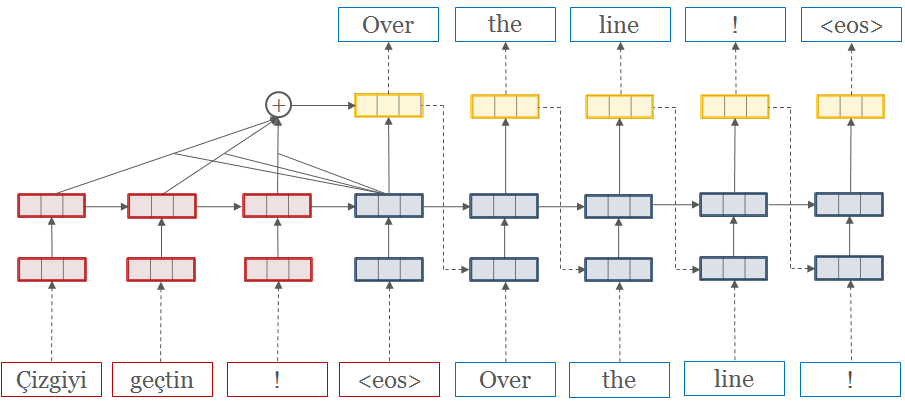
\includegraphics[scale=1]{images/simple-attn.png}
\caption{Neural Machine Translation with attention ({\tiny Image from opennmt.net})}
\end{center}
\end{figure}

%%%%%%%%%%%%%%%%%%%%%%%%%%%%%%%%%%%%%%%%%%%%%%%%%%%%%%%%%%%%%%%%%%%%%%%%%%%%
\slide{Neural Machine Translation in 2015}
\begin{figure}
\begin{center}
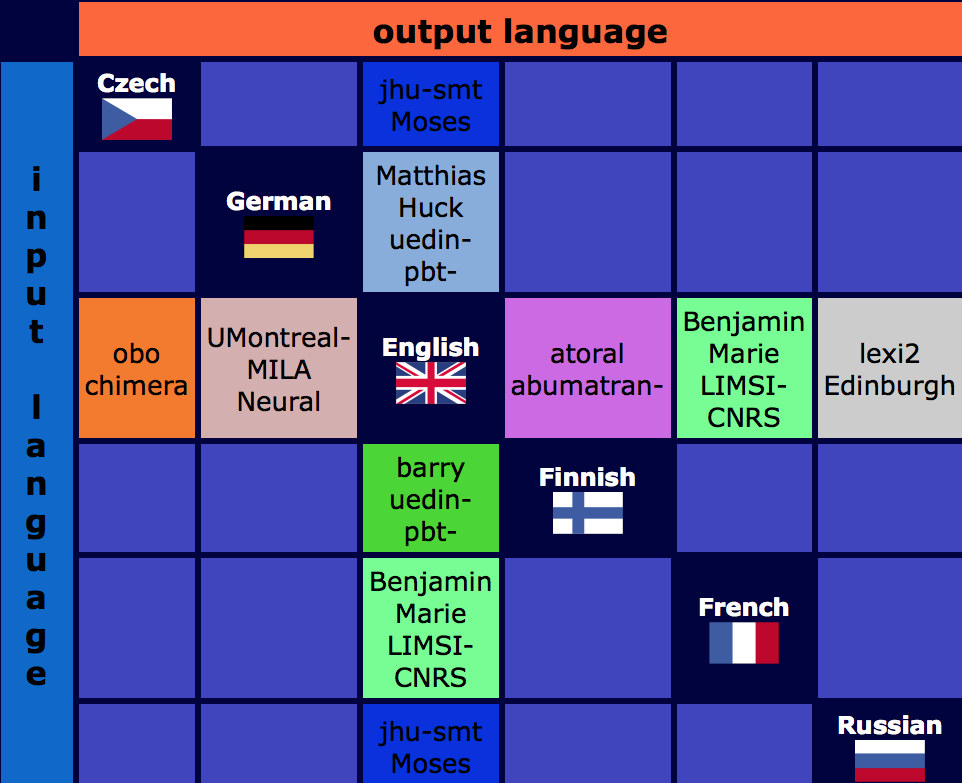
\includegraphics[scale=0.5]{images/n2015.png}
\caption{WMT2015 evaluation results for language-pairs ({\tiny Image from matrix.statmt.org})}
\end{center}
\end{figure}

%%%%%%%%%%%%%%%%%%%%%%%%%%%%%%%%%%%%%%%%%%%%%%%%%%%%%%%%%%%%%%%%%%%%%%%%%%%%
\slide{Neural Machine Translation in 2016}
\begin{figure}
\begin{center}
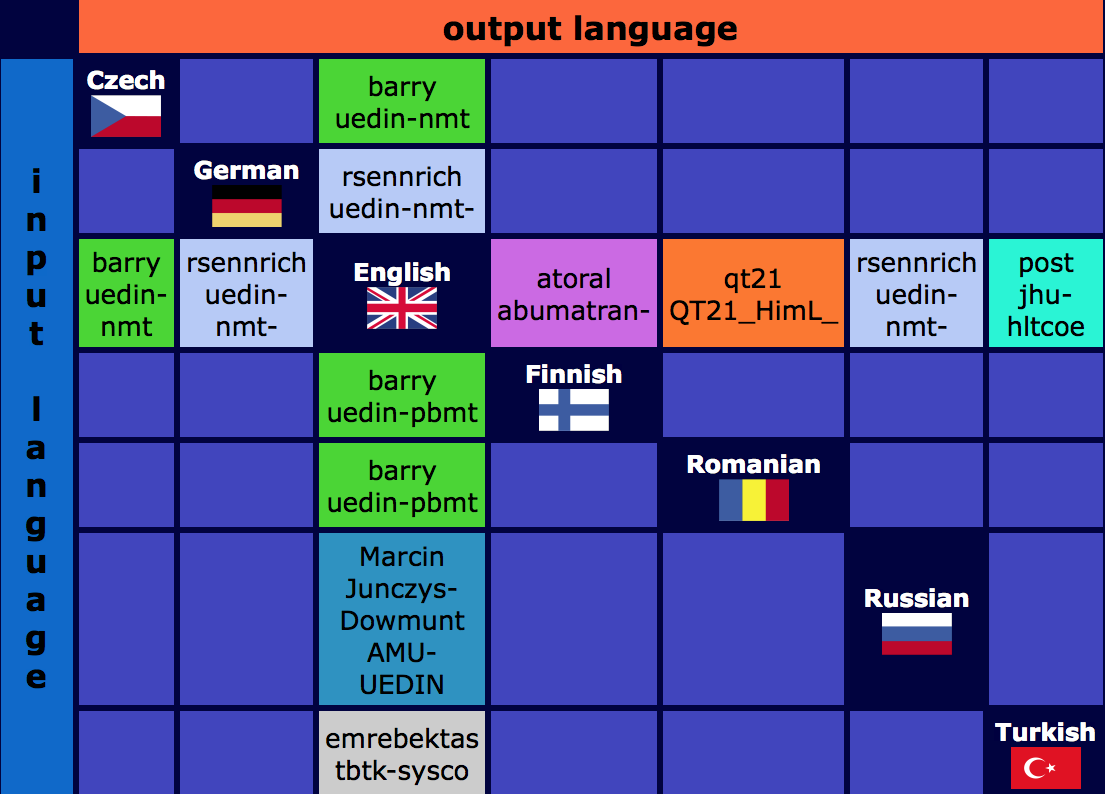
\includegraphics[scale=0.5]{images/n2016.png}
\caption{WMT2016 evaluation results for language-pairs ({\tiny Image from matrix.statmt.org})}
\end{center}
\end{figure}

%%%%%%%%%%%%%%%%%%%%%%%%%%%%%%%%%%%%%%%%%%%%%%%%%%%%%%%%%%%%%%%%%%%%%%%%%%%%
\slide{Are we done?}
\begin{itemize}
\item As more and more parallel data becomes available, the performance of the NMT systems is only going to improve.
\item Research into using monolingual data is already proving successful (TODO: citation here).
\item More complex encoder-decoder models are being proposed every week.
\item Hardware scaling helps supports more parameters and more complex models.
\end{itemize}
\textbf{When does NMT not perform well?}

%%%%%%%%%%%%%%%%%%%%%%%%%%%%%%%%%%%%%%%%%%%%%%%%%%%%%%%%%%%%%%%%%%%%%%%%%%%%
\slide{NMT Challenges : Low Resource}
\begin{figure}
\begin{center}
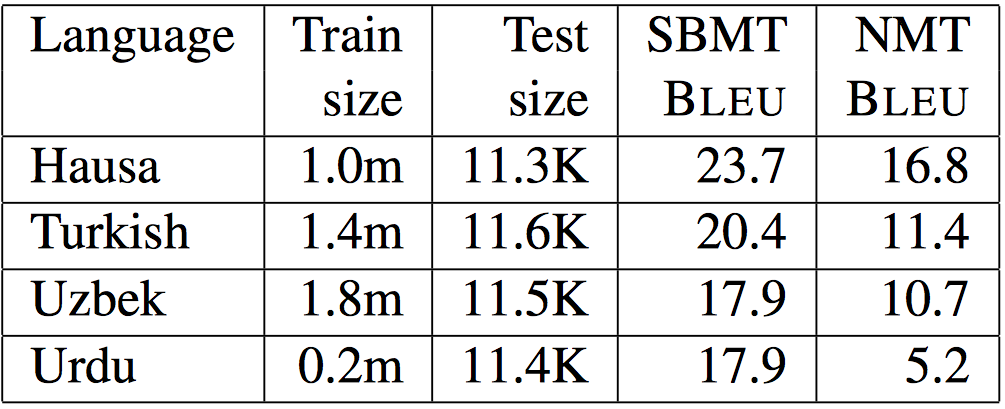
\includegraphics[scale=0.5]{images/low-res.png}
\caption{Performance of NMT models vs. string-to-tree models for low resource languages ({\tiny Image Zoph et al., 2016})}
\end{center}
\end{figure}
Current research
\begin{itemize}
\item Transfer learning : Zoph et al., 2016
\item Multi-way, multi-lingual NMT : Firat et al., 2016
\end{itemize}

%%%%%%%%%%%%%%%%%%%%%%%%%%%%%%%%%%%%%%%%%%%%%%%%%%%%%%%%%%%%%%%%%%%%%%%%%%%%
\slide{NMT Challenges : Out of domain}
\begin{itemize}
\item A problem not unique to NMT
\item A fundamental challenge for DARPA Lorelei
\item Assume that you have access to parallel text in the following domains: religious, legal and IT. Your job is to come up with a translation system that can be used to assist and converse with earthquake victims.
\item Possibly worse for NMT because of the drastically different style of writing used in the out of domain training text. This is the trouble with using source conditioned language models.
\end{itemize}

\slide{NMT Challenges : Out of domain}
\vspace{10mm}
\begin{center}
\begin{tabular}{l|r|r|r|r|r}
\bf System & \multicolumn{1}{c|}{\bf Law} & \multicolumn{1}{c|}{\bf Medical} & \multicolumn{1}{c|}{\bf IT} & \multicolumn{1}{c|}{\bf Koran} & \multicolumn{1}{c}{\bf Subtitles} \\ \hline
All & \textcolor{red}{--1.3} & \textcolor{darkgreen}{+2.9} & \textcolor{red}{--9.4} & $\pm$0.0 & \textcolor{darkgreen}{+5.6} \\ \hline
Law & \textcolor{red}{--3.3} & \textcolor{red}{--6.1} & \textcolor{red}{--3.4} & \textcolor{red}{--0.9} & \textcolor{red}{--3.2}\\ 
Medical & \textcolor{red}{--6.3} & \textcolor{red}{--4.1} & \textcolor{red}{--6.5} & \textcolor{red}{--1.4} & \textcolor{red}{--4.4} \\
IT & \textcolor{red}{--1.8} & \textcolor{red}{--1.2} & \textcolor{darkgreen}{+2.3} & \textcolor{darkgreen}{+0.2 } & \textcolor{red}{--0.8} \\
Koran & \textcolor{red}{--1.4} & \textcolor{red}{--2.1} & \textcolor{red}{--2.3} & \textcolor{red}{--2.9} & \textcolor{red}{--4.5} \\
Subtitles & \textcolor{red}{--2.9} & \textcolor{red}{--8.5} & \textcolor{red}{--4.4} & \textcolor{darkgreen}{+0.6} &  \textcolor{darkgreen}{+3.8} \\
\end{tabular}
\captionof{table}{Relative performance of NMT systems with respect to PBMT systems for out-of-domain test sets in German-English ({\tiny From Philipp Koehn})} 
\end{center}

%%%%%%%%%%%%%%%%%%%%%%%%%%%%%%%%%%%%%%%%%%%%%%%%%%%%%%%%%%%%%%%%%%%%%%%%%%%%
\slide{NMT Challenges : The UNK problem}
\begin{itemize}
	\item NMT sytems do not copy words from the source into the target if an unknown word is encountered. 	\item For languages which have a large vocabulary size or greater morphological complexity, producing an UNK is safe
	\item Degenerate solution, if enough UNKs are in the training data, safely produce an UNK during translation
\end{itemize}

\vspace{1mm}
An example from Romanian-English (newstest2016):\\
\textbf{Ref} : 46 percent said they are leaving the door open to switching candidates .\\
\textbf{Moses} : \textcolor{verydarkorange}{46 \% say porti?a leaves open the possibility of changing the option .}\\
\textbf{NMT} : \textcolor{darkgreen}{46 per cent affirmative the \textbf{unk} tag \# sel\textbf{unk} tag \# sel\textbf{unk}}\\

%%%%%%%%%%%%%%%%%%%%%%%%%%%%%%%%%%%%%%%%%%%%%%%%%%%%%%%%%%%%%%%%%%%%%%%%%%%%
\slide{NMT Challenges : The rare word problem}
\begin{figure}
\begin{center}
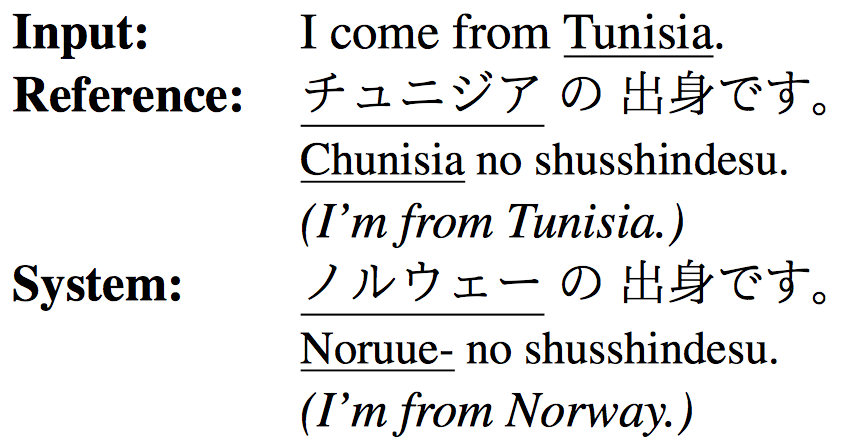
\includegraphics[scale=0.3]{images/rare.png}
\caption{A mistake made by an NMT system on a low-frequency content word ({\tiny Image from Arthur et al., 2016})}
\end{center}
\end{figure}
\begin{itemize}
\item Rare words which belong to a common word class are often confused.
\item This problem is worse for words that are of interest for downstream NLP tasks such as NER.
\end{itemize}

%%%%%%%%%%%%%%%%%%%%%%%%%%%%%%%%%%%%%%%%%%%%%%%%%%%%%%%%%%%%%%%%%%%%%%%%%%%%
\slide{NMT Challenges : The rare word problem}
\vspace{10mm}
Current Research
\begin{itemize}
\item Subword translation (Sennrich et al., 2015)
\item Character level NMT (Ling et al., 2015)
\item Incorporations of lexicons (Arthur et al., 2016)
\item Tracking source words which produced OOVs (Luong et al., 2015)
\end{itemize}

%%%%%%%%%%%%%%%%%%%%%%%%%%%%%%%%%%%%%%%%%%%%%%%%%%%%%%%%%%%%%%%%%%%%%%%%%%%%
\slide{NMT Challenges : Length ratios \& hallucination}
\vspace{10mm}
\begin{center}
\begin{tabular}{|p{3cm}|p{20cm}|}
\textbf{Ref} & ban urged the five permanent members to show the solidarity and unity they did in achieving an iran nuclear deal in addressing the syria crisis .\\[1cm] \hline \hline
\textbf{Moses} & \textcolor{verydarkorange}{ban urged the five permanent members to show solidarity and unity shown when they failed to reach a deal on iran 's nuclear weapons , thus addressing the crisis in syria .} \\[1cm] \hline \hline
\textbf{NMT} & \textcolor{darkgreen}{ban called on the five permanent members of the lib dems to give \textbf{pumpkins of solidarity with the arthritis unit} , then the cudgel reeled it sunk nkey an agreement on iran 's nuclear weapons , to handle the crisis in syria .}
\end{tabular}
\captionof{table}{An example translation from the Romanian-English newstest2016 test set.} 
\end{center}



%%%%%%%%%%%%%%%%%%%%%%%%%%%%%%%%%%%%%%%%%%%%%%%%%%%%%%%%%%%%%%%%%%%%%%%%%%%%
\slide{NMT Challenges : Ignoring source context}
\begin{itemize}
\item No explicit accountability for translating all source words with NMT models
\end{itemize}
\begin{figure}
\begin{center}
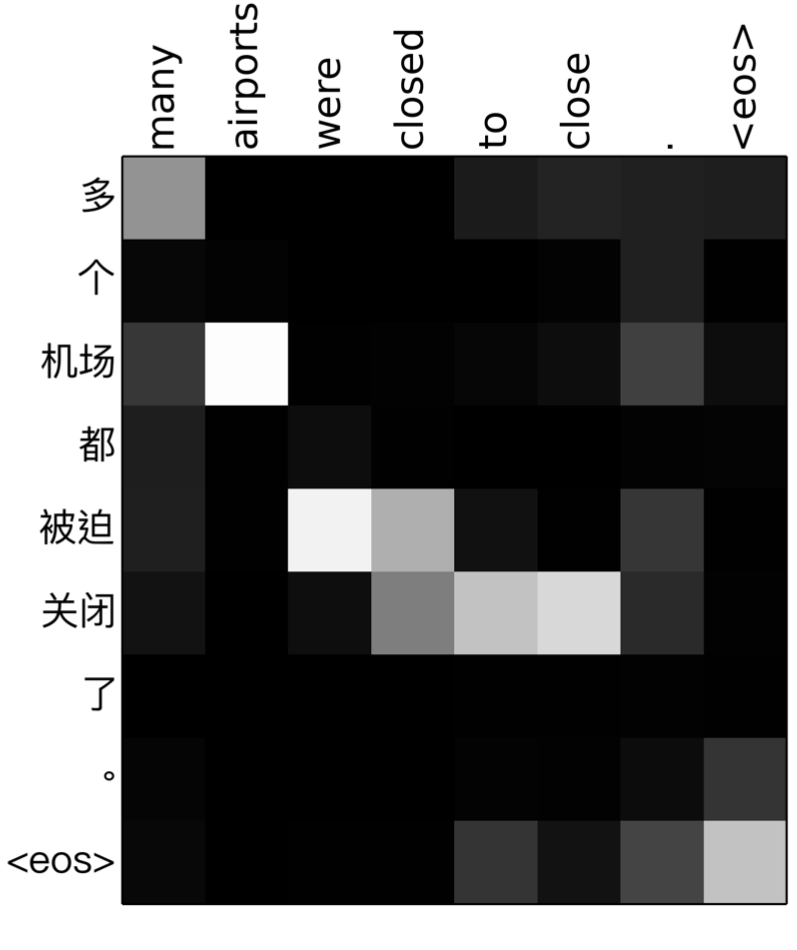
\includegraphics[scale=0.2]{images/coverage.png}
\caption{Ignoring source words in translation with NMT models ({\tiny Image from Tu et al., 2016})}
\end{center}
\end{figure}
Current Research: 
\begin{itemize}
\item Modeling coverage vectors (Tu et al., 2016, Mi et al., 2016)
\item Supervised alignments (Liu et al., 2016)
\end{itemize}

%%%%%%%%%%%%%%%%%%%%%%%%%%%%%%%%%%%%%%%%%%%%%%%%%%%%%%%%%%%%%%%%%%%%%%%%%%%%
\slide{Adequacy vs. Fluency}
\begin{itemize}
\item SMT systems are tasked with the explicit translation of each component within the source sentence (\textbf{adequate}).
\item NMT systems produce text which is generally fluent and fairly well conditioned on the source sentence (\textbf{fluent}).
\end{itemize}

We plan to combine these benefits by using the SMT system to \textbf{constrain the hypothesis space of adequate translations} available to the NMT system which will choose the most fluent one.

%%%%%%%%%%%%%%%%%%%%%%%%%%%%%%%%%%%%%%%%%%%%%%%%%%%%%%%%%%%%%%%%%%%%%%%%%%%%
\slide{Related work}
\begin{itemize}
\item \textbf{System combination} : Using $n$-best lists for combination (via features or otherwise) for multiple NMT and SMT systems if common.
\item \textbf{Moses with NMT features} : Use the NMT score as a feature in PBMT (Junczys-Dowmunt et al., 2016).
\item \textbf{Promoting diversity in beam search} (Vijayakumar et al., 2016) 
\item \textbf{Using alternate objective functions} while training NMT systems to increase diversity (Li et al., 2016)
\item \textbf{Minimize Bayes risk with respect to lattices} (Stahlberg et al., 2017)
\end{itemize}


%%%%%%%%%%%%%%%%%%%%%%%%%%%%%%%%%%%%%%%%%%%%%%%%%%%%%%%%%%%%%%%%%%%%%%%%%%%%
\slide{SMT Search graphs}
\begin{figure}
\begin{center}
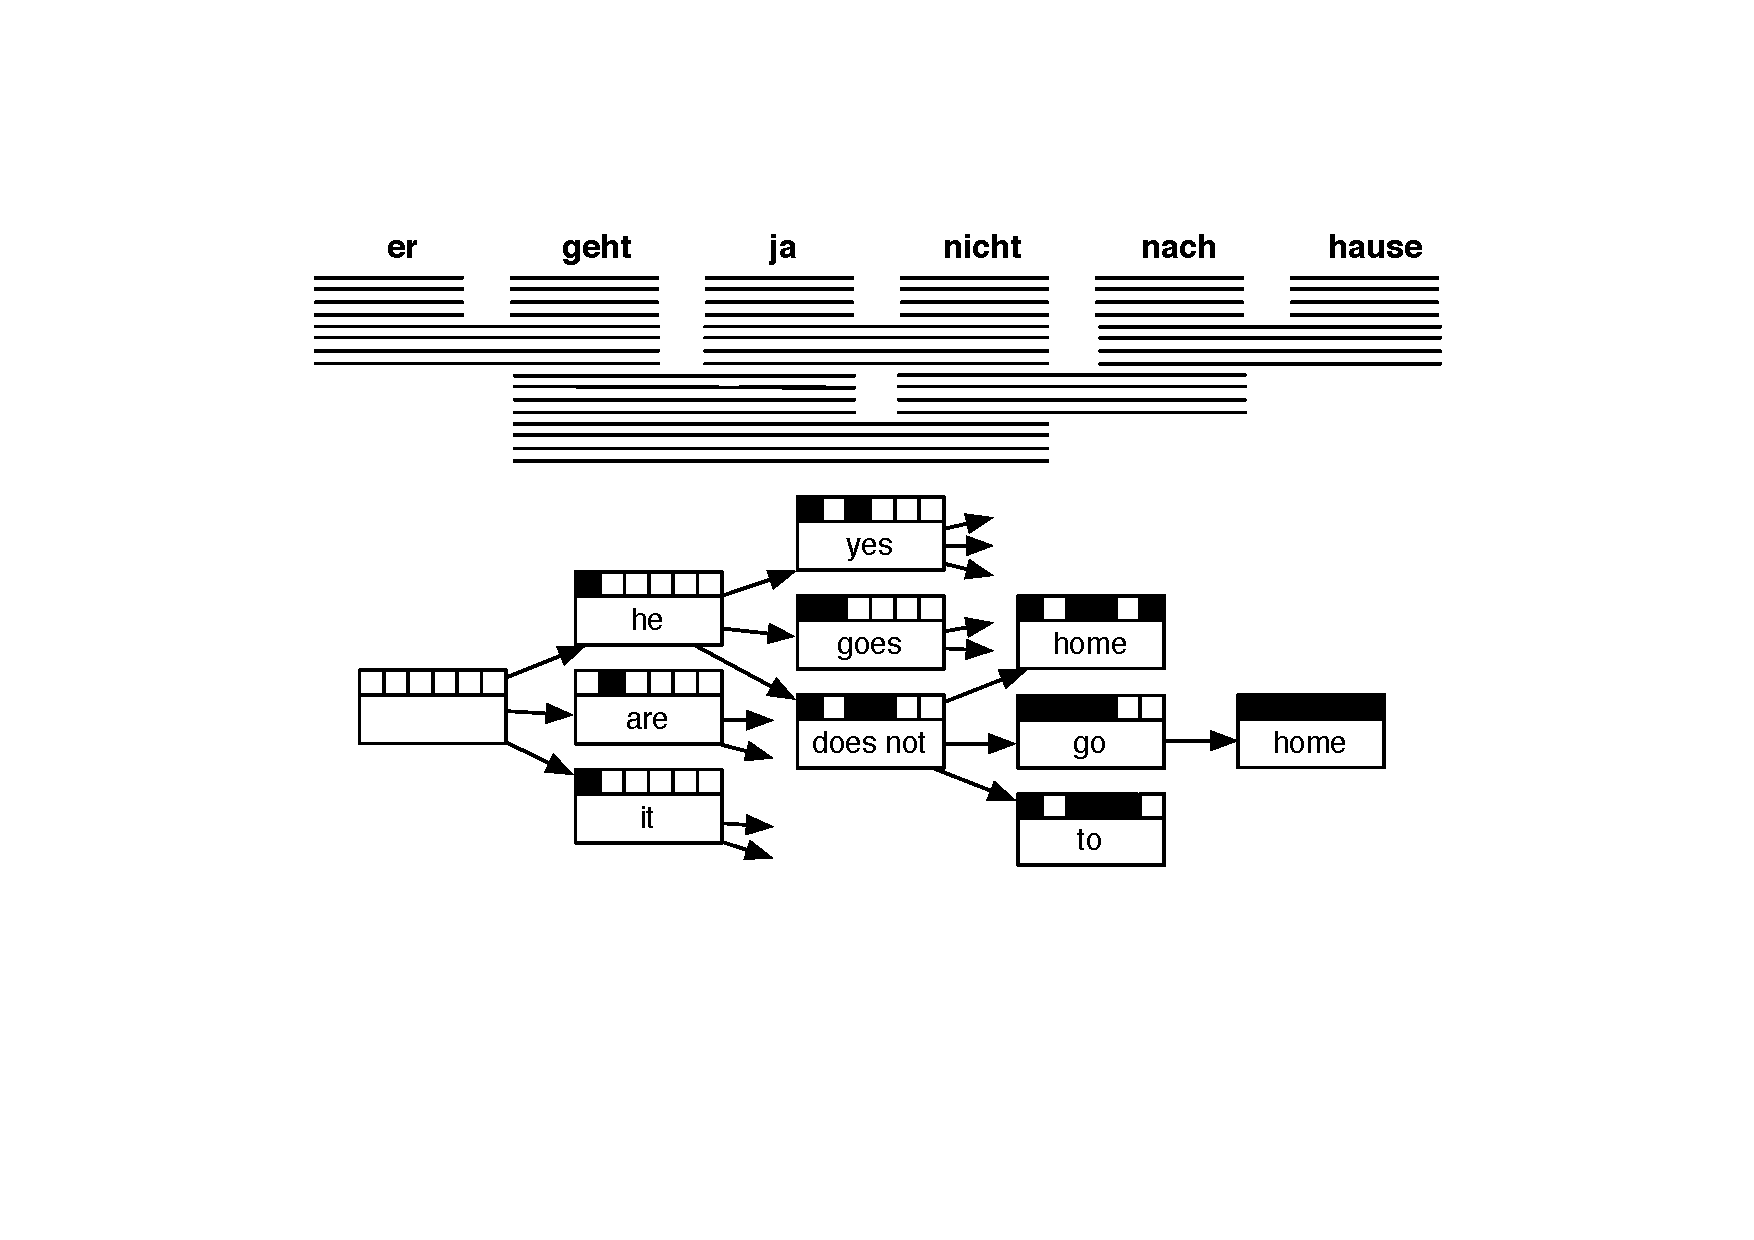
\includegraphics[scale=1.2]{images/graph.pdf}
%\caption{Neural Machine Translation with attention ({\tiny Image from opennmt.net})}
\end{center}
\end{figure}

%%%%%%%%%%%%%%%%%%%%%%%%%%%%%%%%%%%%%%%%%%%%%%%%%%%%%%%%%%%%%%%%%%%%%%%%%%%%
\slide{Re-scoring SMT Search graphs}
\begin{itemize}
\item Search graphs (which can be converted to word lattices) represent a compact and potentially diverse set of translation hypotheses.
\item	In comparison, $n$-best lists may lack this diversity.
\item Search graphs also allow efficient traversal of the hypothesis space, eliminating entire sub-graphs of translations if their prefix scores are bad. This is not possible with $n$-best lists.
\item For this study, we limit the role of the SMT system to constraining the search space. We discard all of the SMT features and scores on the lattice.
\item Out-of-domain neural models are useful again, since they are choosing from a constrained adequate hypothesis space.
\end{itemize}

%%%%%%%%%%%%%%%%%%%%%%%%%%%%%%%%%%%%%%%%%%%%%%%%%%%%%%%%%%%%%%%%%%%%%%%%%%%%
\slide{Stack-based re-scoring algorithm}
\begin{figure}
\begin{center}
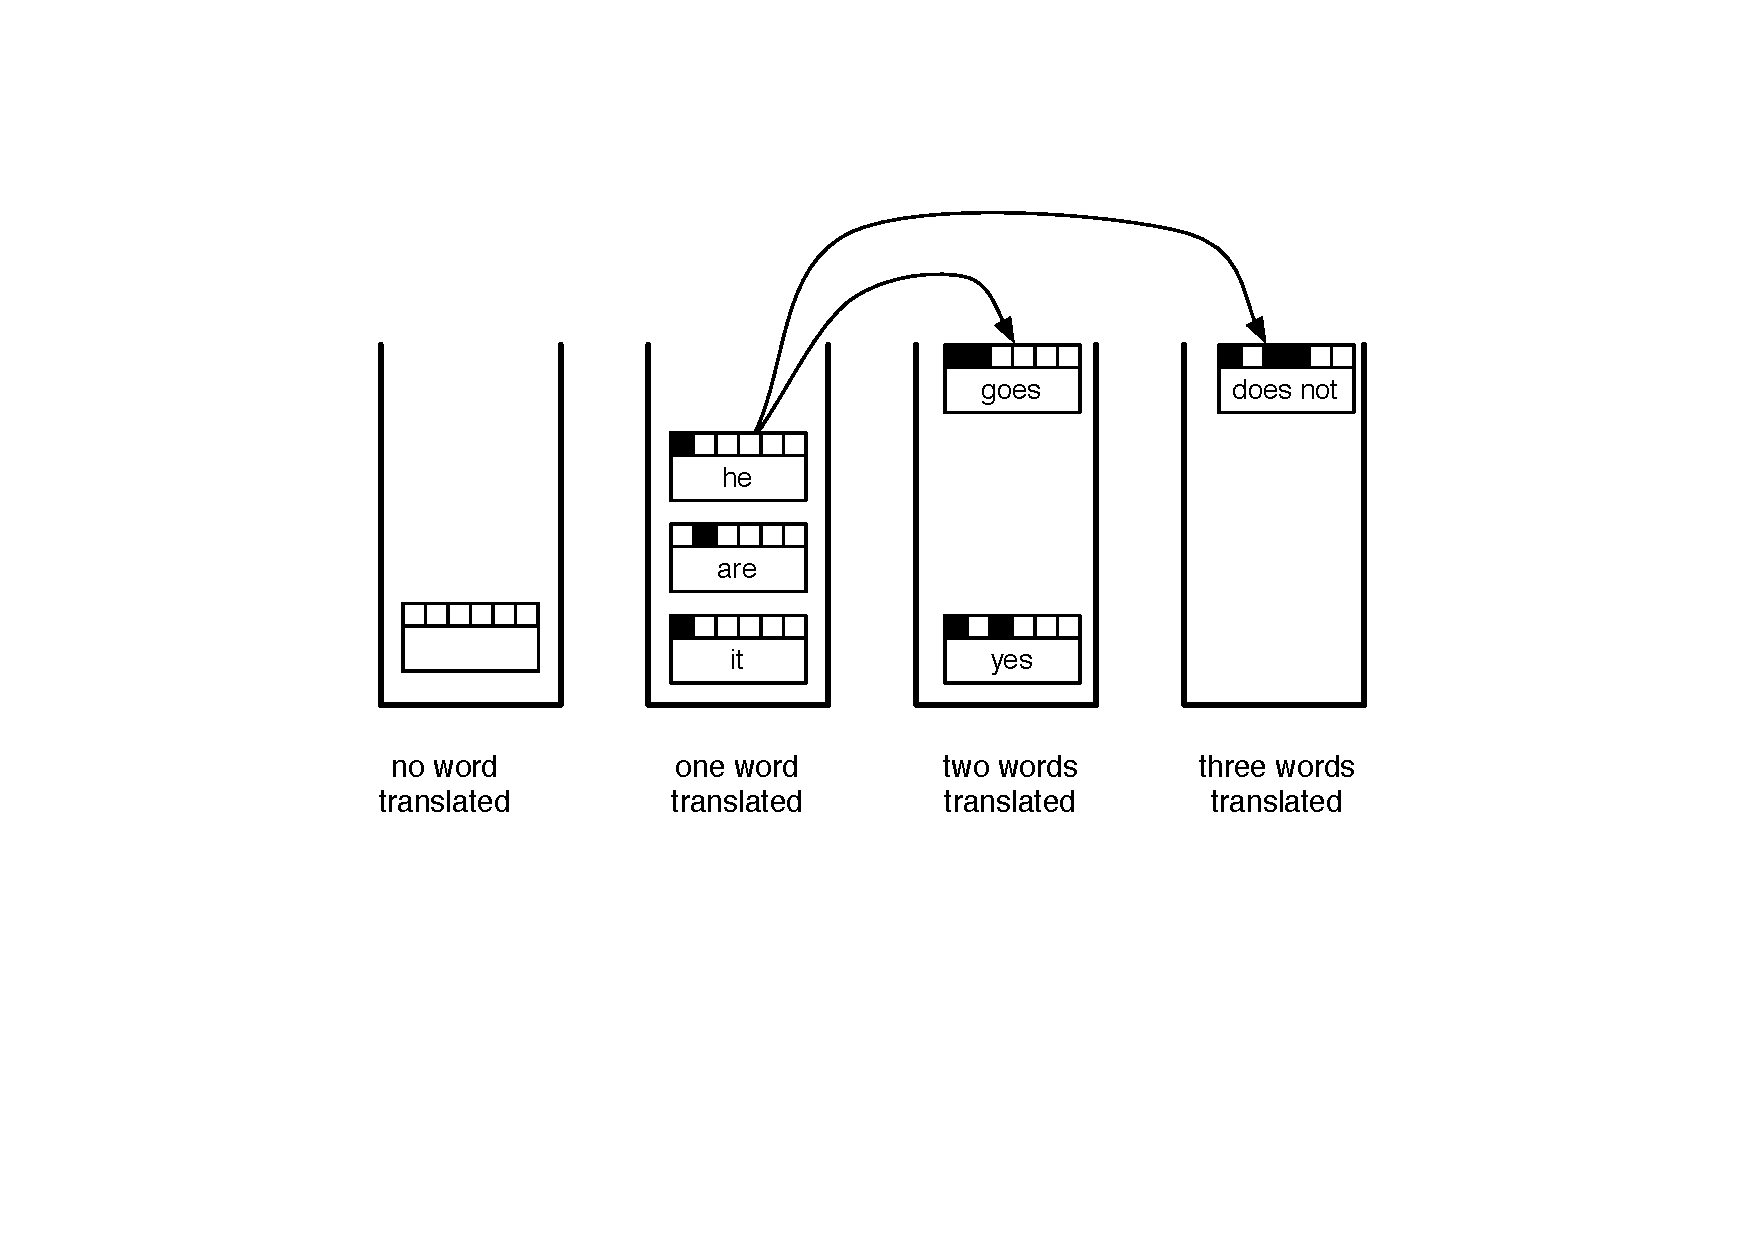
\includegraphics[scale=1.2]{images/stack1.pdf}
\caption{Phrase based stack decoding ({\tiny Image from Philipp Koehn})}
\end{center}
\end{figure}

%%%%%%%%%%%%%%%%%%%%%%%%%%%%%%%%%%%%%%%%%%%%%%%%%%%%%%%%%%%%%%%%%%%%%%%%%%%%
\slide{Stack-based re-scoring algorithm}
\begin{figure}
\begin{center}
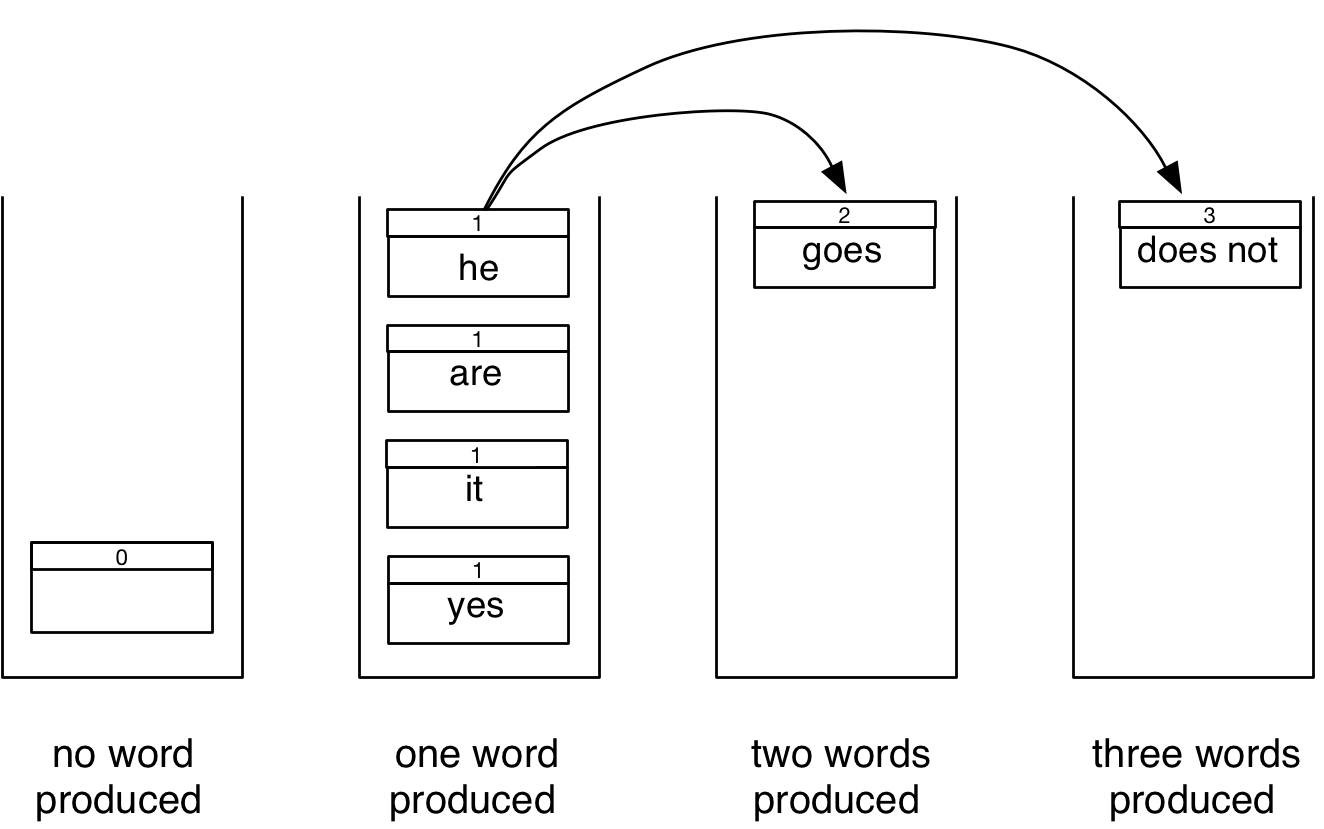
\includegraphics[scale=0.3]{images/stack2.png}
\caption{Search graph stack rescoring}
\end{center}
\end{figure}
\begin{itemize}
\item All complete hypotheses are moved to a ``complete'' stack.
\item All scores are length normalized to avoid a length bias.
\end{itemize}

%%%%%%%%%%%%%%%%%%%%%%%%%%%%%%%%%%%%%%%%%%%%%%%%%%%%%%%%%%%%%%%%%%%%%%%%%%%%
\slide{Recombination}
\begin{figure}
\begin{center}
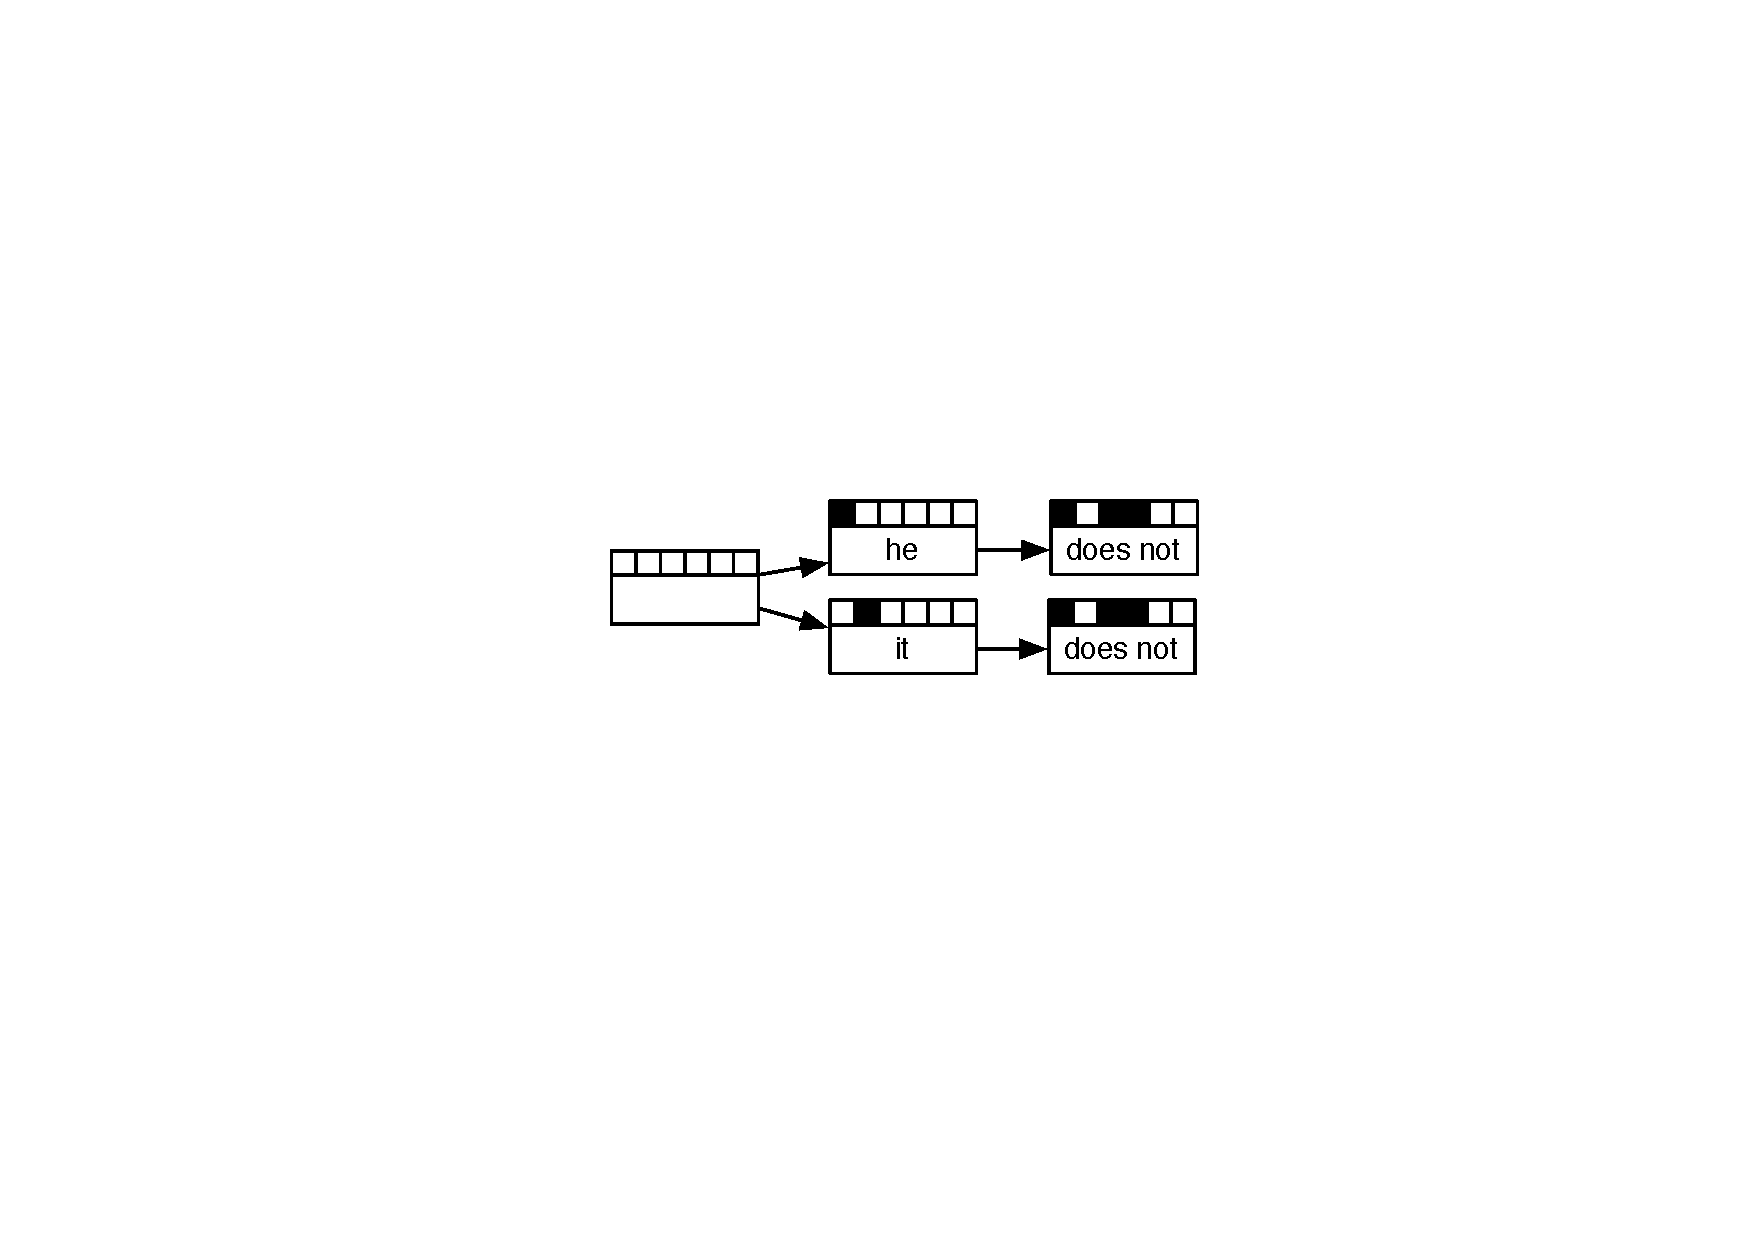
\includegraphics[scale=1]{images/recombination1.pdf}\\
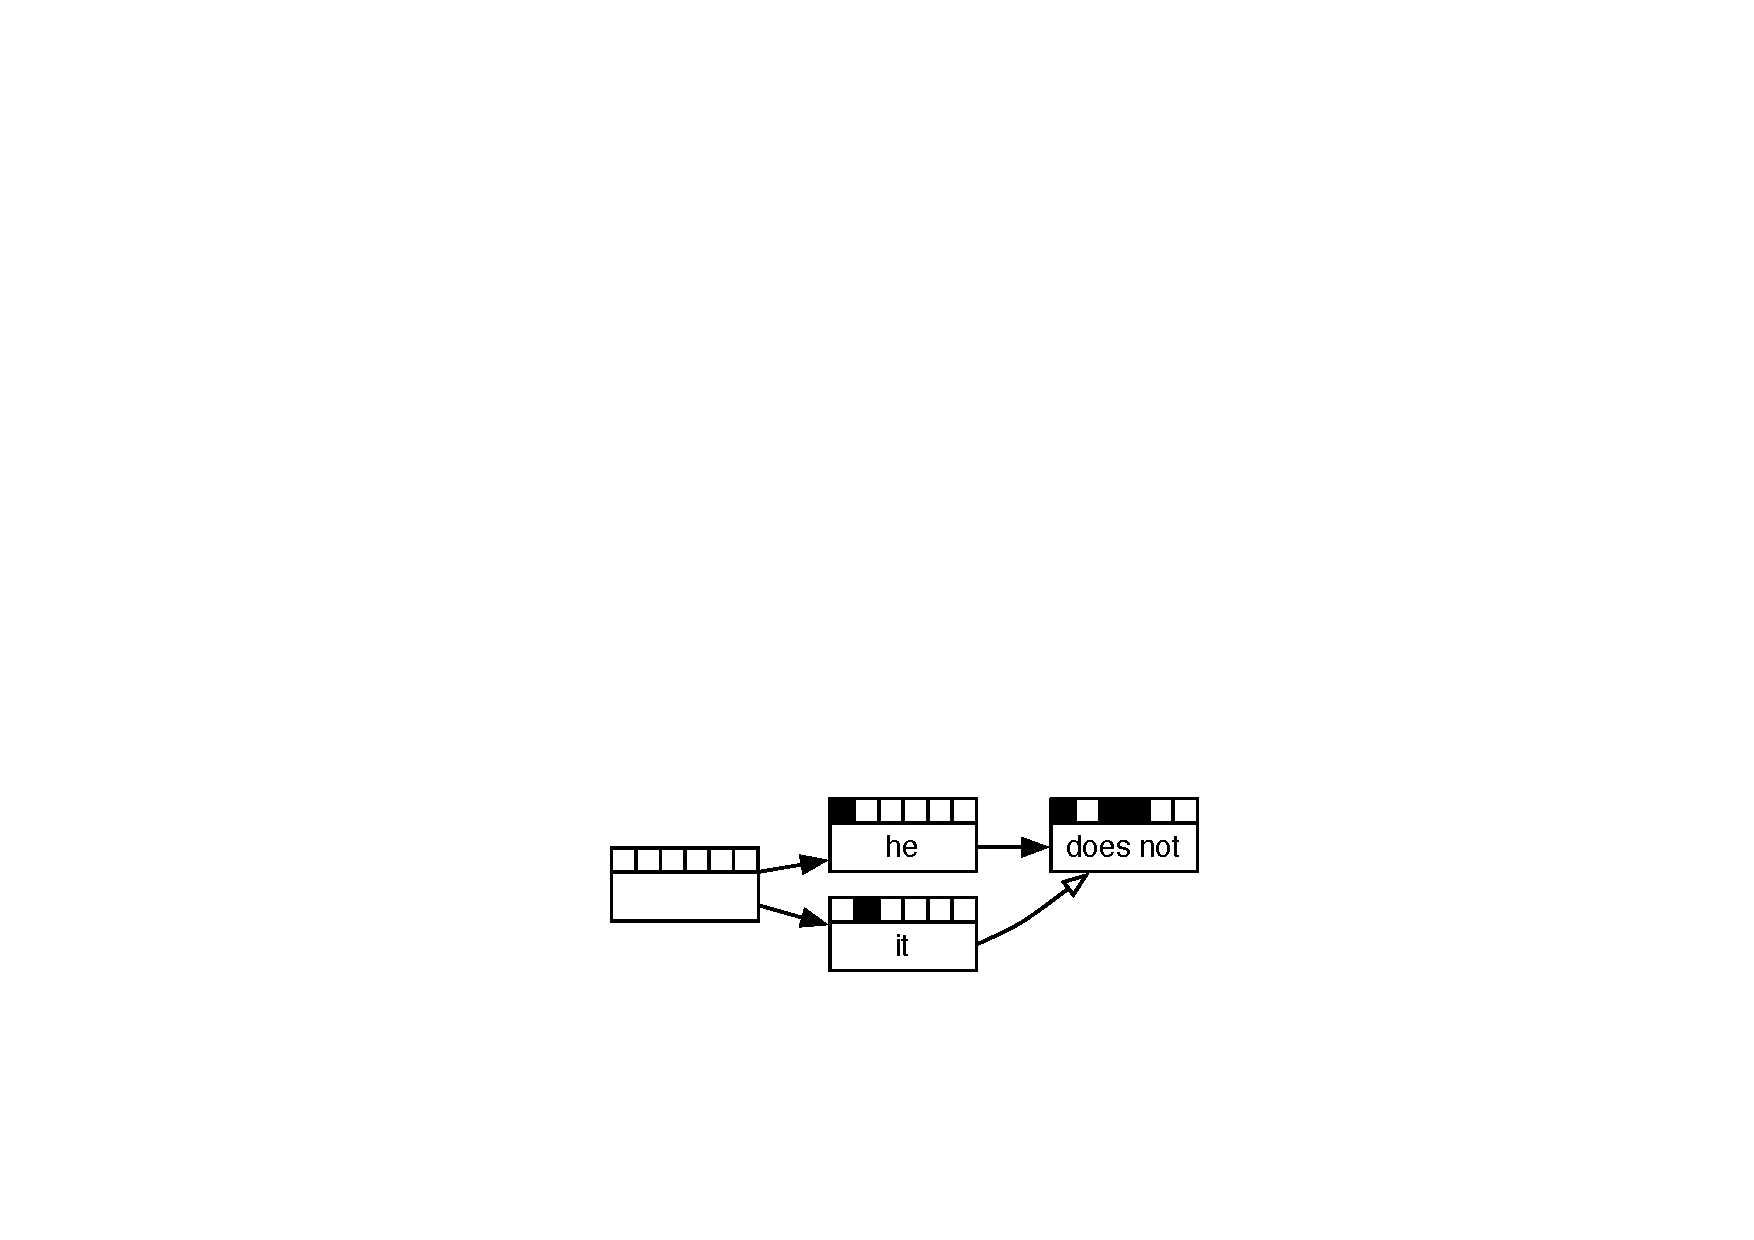
\includegraphics[scale=1]{images/recombination2.pdf}
\caption{Recombination in a search graph when the states are indistinguishable.}
\end{center}
\end{figure}
\begin{itemize}
\item When states in a search graph are indistinguishable with respect to their contexts but have different scores.
\item Drop the worse one in a traditional SMT stack decoder.
\item How do we handle this with NMT re-scoring, since each path has a unique context?
\end{itemize}

%%%%%%%%%%%%%%%%%%%%%%%%%%%%%%%%%%%%%%%%%%%%%%%%%%%%%%%%%%%%%%%%%%%%%%%%%%%%
\slide{Recombination}
\vspace{10mm}
For lattice re-scoring with stacks:
\begin{itemize}
\item Treat each state in a stack (now, an RNN state) as unique
\item However, only keep the top $k$ entries in a stack when processing it (Histogram pruning)
\item Expand all possibilities from the best $k$ entries of the stack currently being processed.
\end{itemize}

%%%%%%%%%%%%%%%%%%%%%%%%%%%%%%%%%%%%%%%%%%%%%%%%%%%%%%%%%%%%%%%%%%%%%%%%%%%%
\slide{Stack-based re-scoring algorithm}
\begin{itemize}
\item Explores an ``adequate'' hypothesis space of translations with neural translation models.
\item The exploration space is typically more diverse than $n$-best lists.
\item No re-training of the models is required.
\item This is faster than using the NMT feature function in SMT systems.
\item When the SMT system is more robust than the NMT models, this may potentially improve quality.
\end{itemize}

%%%%%%%%%%%%%%%%%%%%%%%%%%%%%%%%%%%%%%%%%%%%%%%%%%%%%%%%%%%%%%%%%%%%%%%%%%%%
\slide{Experiments}
\vspace{10mm}
\begin{itemize}
\item
\item
\end{itemize}
Desc datasets, systems

%%%%%%%%%%%%%%%%%%%%%%%%%%%%%%%%%%%%%%%%%%%%%%%%%%%%%%%%%%%%%%%%%%%%%%%%%%%%
\slide{Results: SMT better, NMT worse}
\begin{figure}
\begin{center}
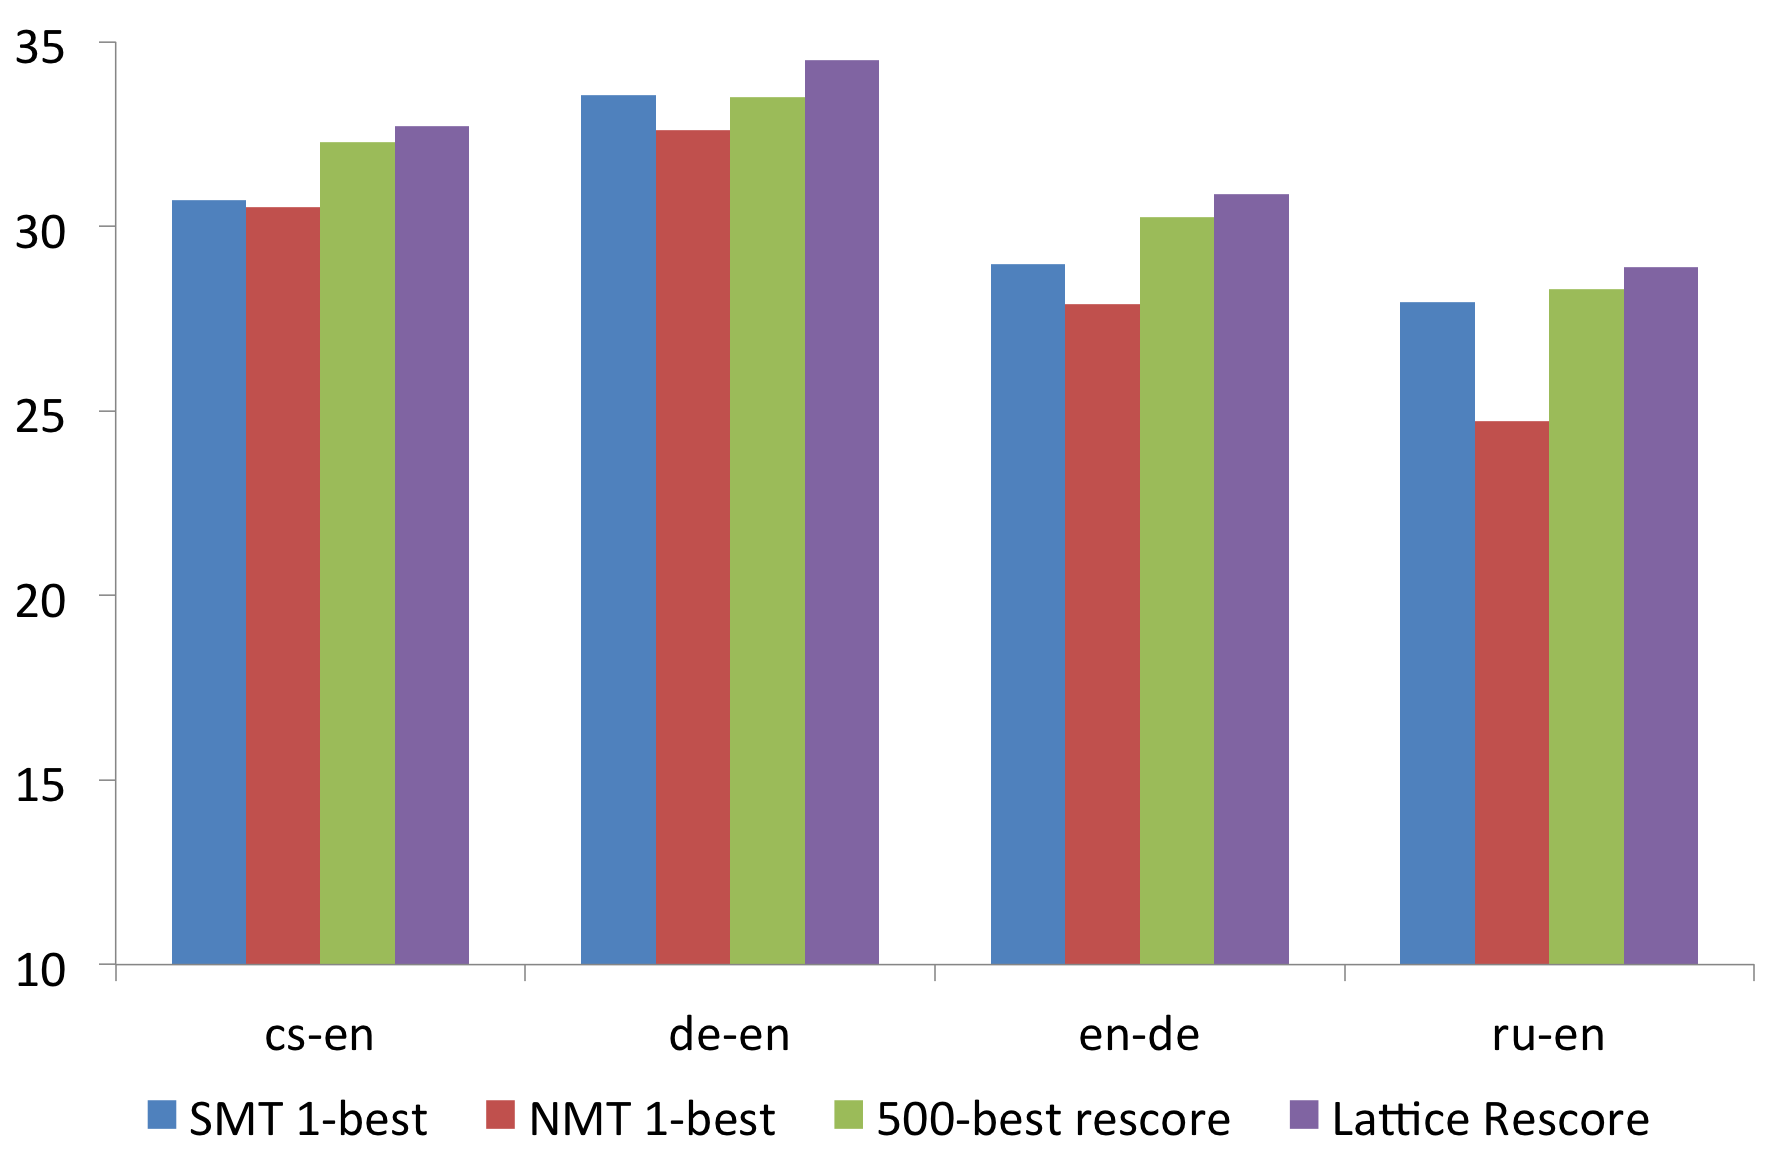
\includegraphics[scale=0.7]{images/smtBetter.png}
\caption{Lattice re-scoring performs the best when SMT is better than NMT.}
\end{center}
\end{figure}

%%%%%%%%%%%%%%%%%%%%%%%%%%%%%%%%%%%%%%%%%%%%%%%%%%%%%%%%%%%%%%%%%%%%%%%%%%%%
\slide{Results: SMT worse, NMT better}
\begin{figure}
\begin{center}
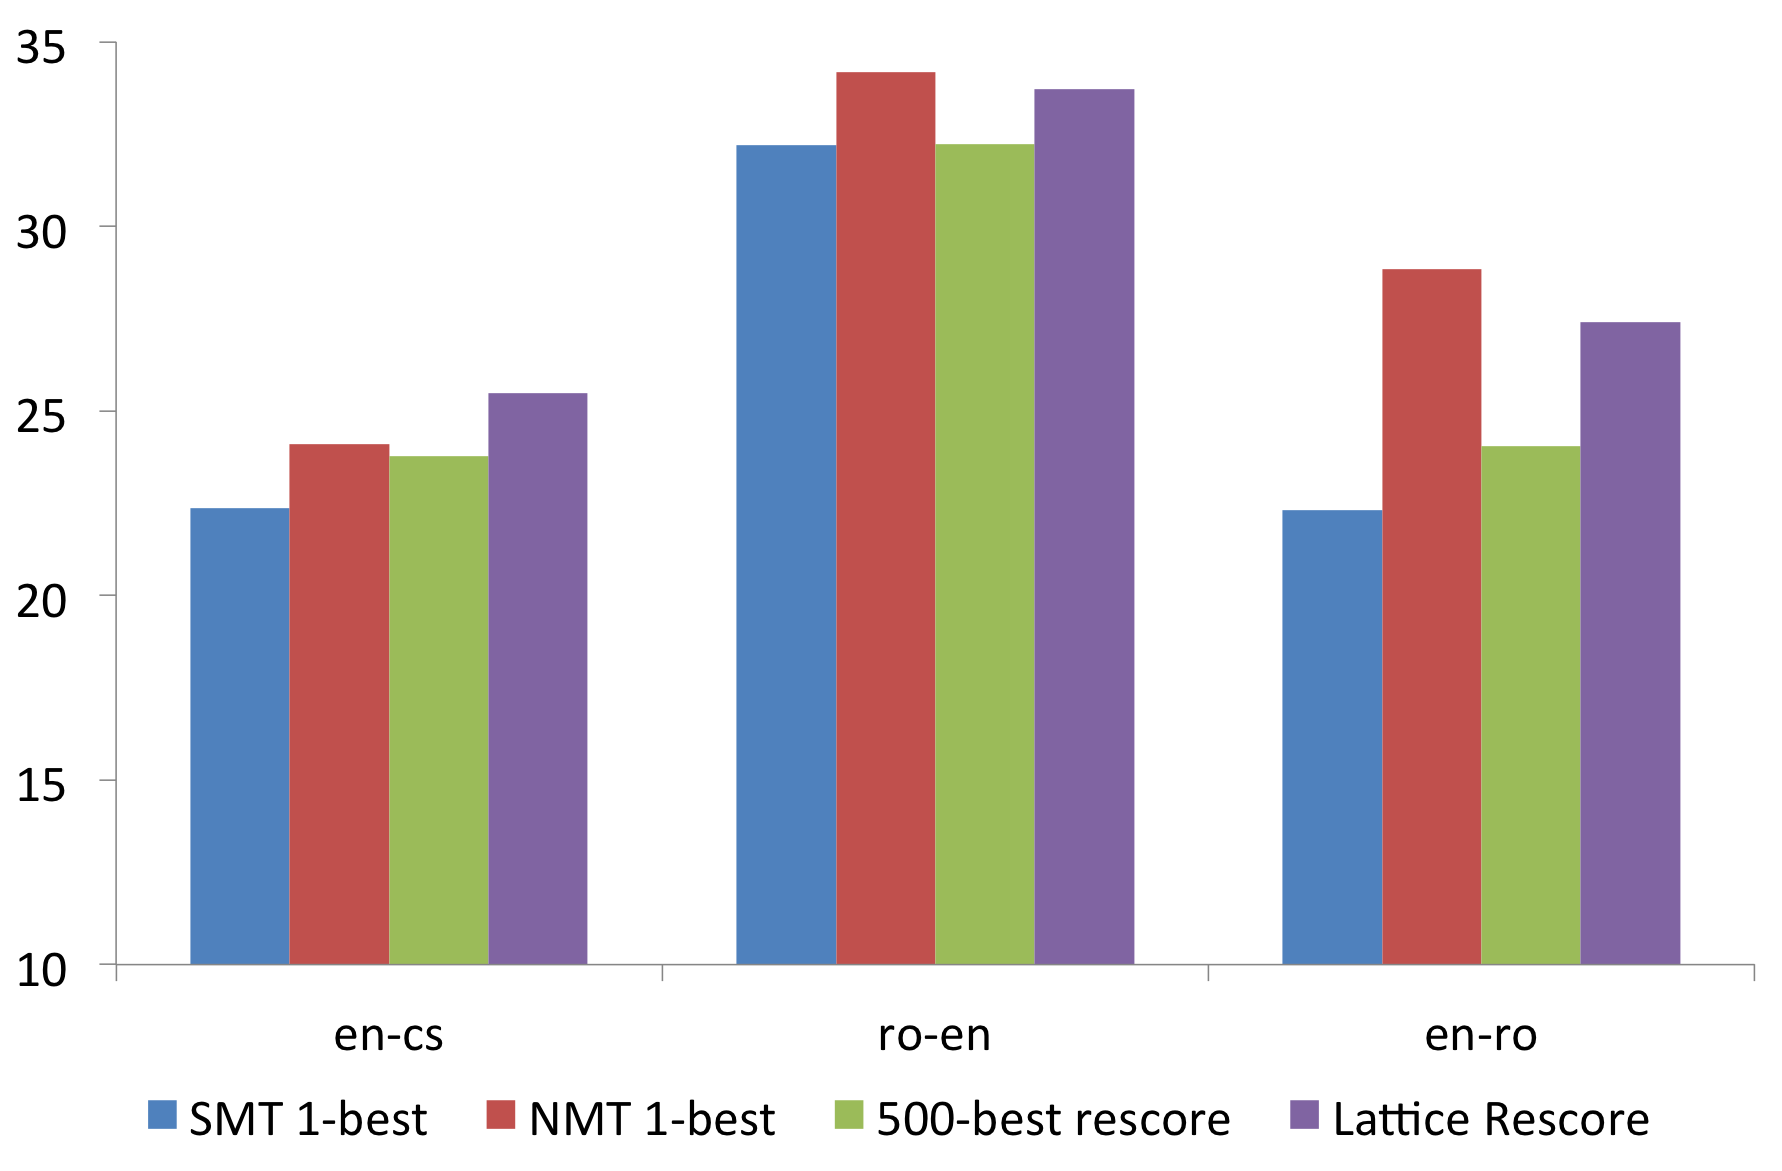
\includegraphics[scale=0.7]{images/nmtBetter.png}
\caption{Lattice re-scoring performance when NMT is better than SMT.}
\end{center}
\end{figure}

%%%%%%%%%%%%%%%%%%%%%%%%%%%%%%%%%%%%%%%%%%%%%%%%%%%%%%%%%%%%%%%%%%%%%%%%%%%%
\slide{The effect of pruning}
\begin{figure}
\begin{center}
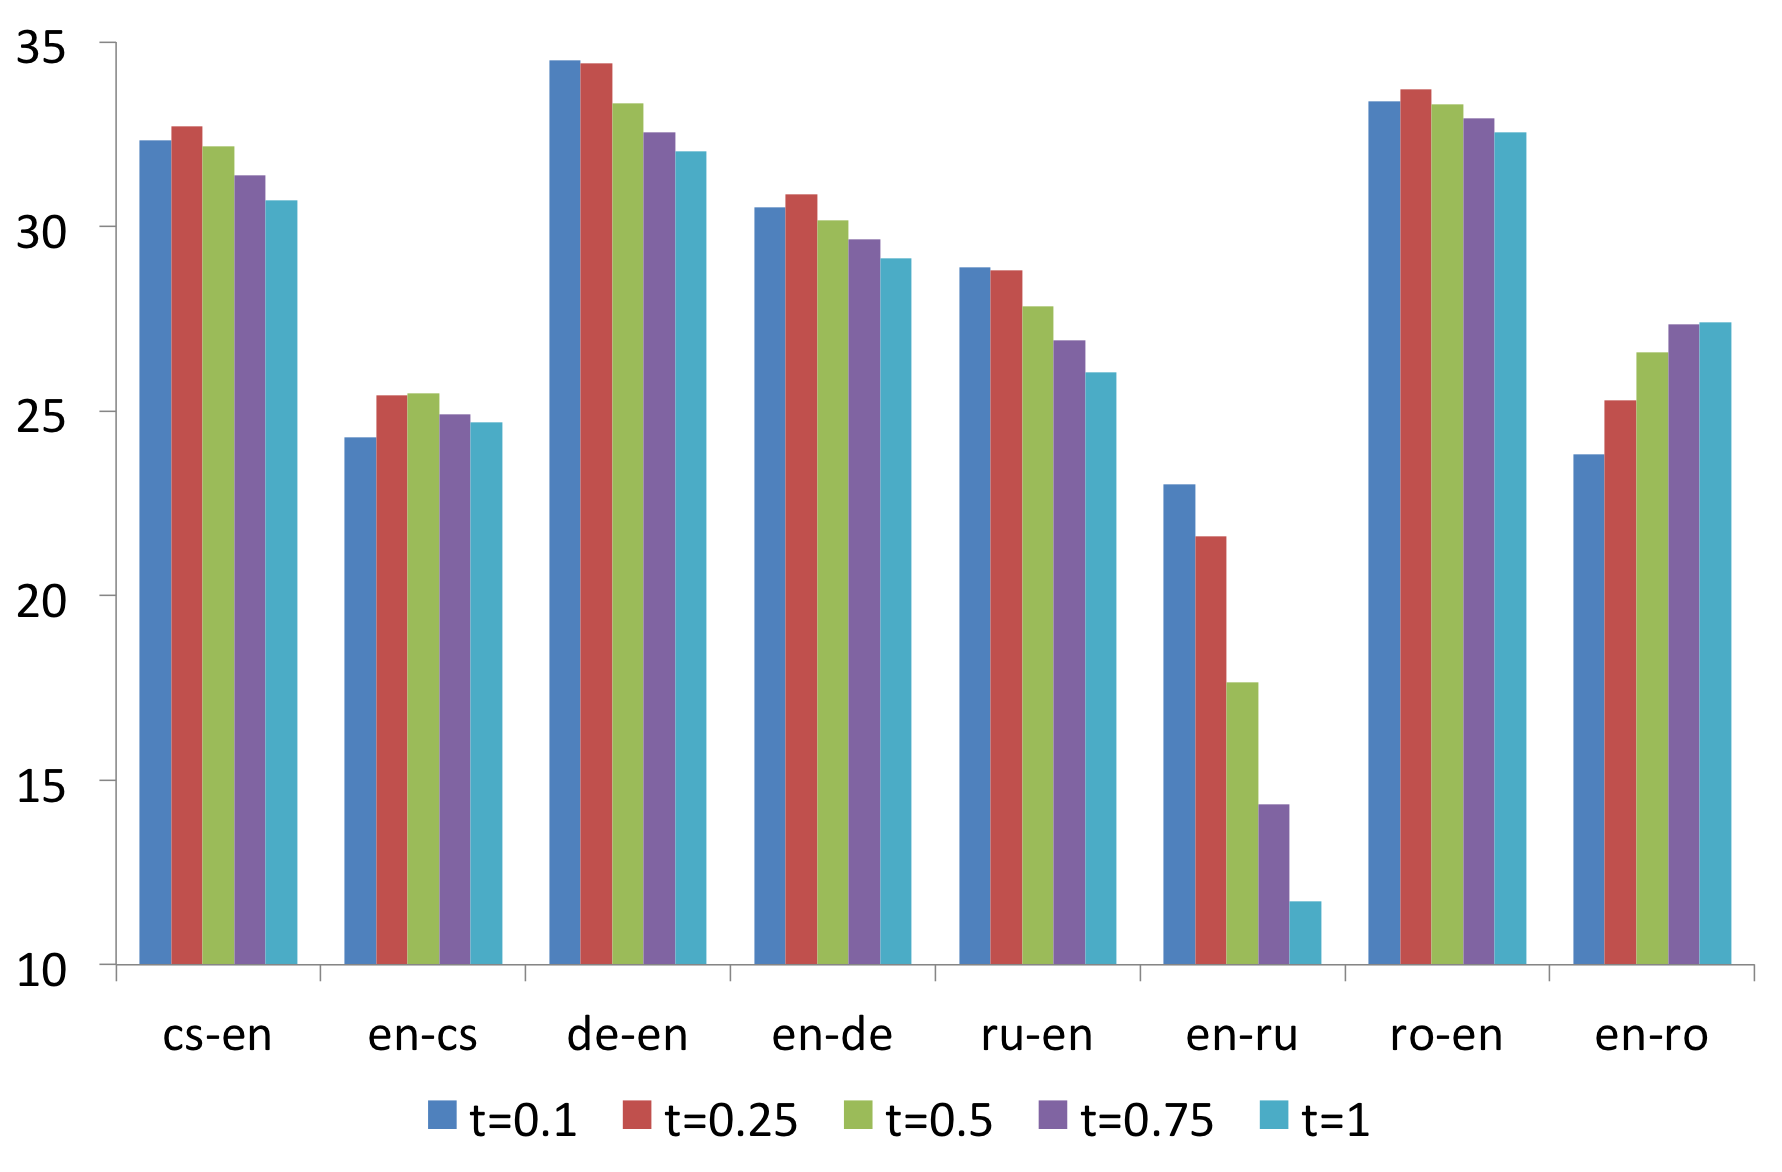
\includegraphics[scale=0.7]{images/thresholds.png}
\caption{}
\end{center}
\end{figure}

%%%%%%%%%%%%%%%%%%%%%%%%%%%%%%%%%%%%%%%%%%%%%%%%%%%%%%%%%%%%%%%%%%%%%%%%%%%%
\slide{Domain Adaptation, Low Resource}
Graphs here

\end{document}